\subsection{Lock}

\begin{figure}[htbp]
   \centering
   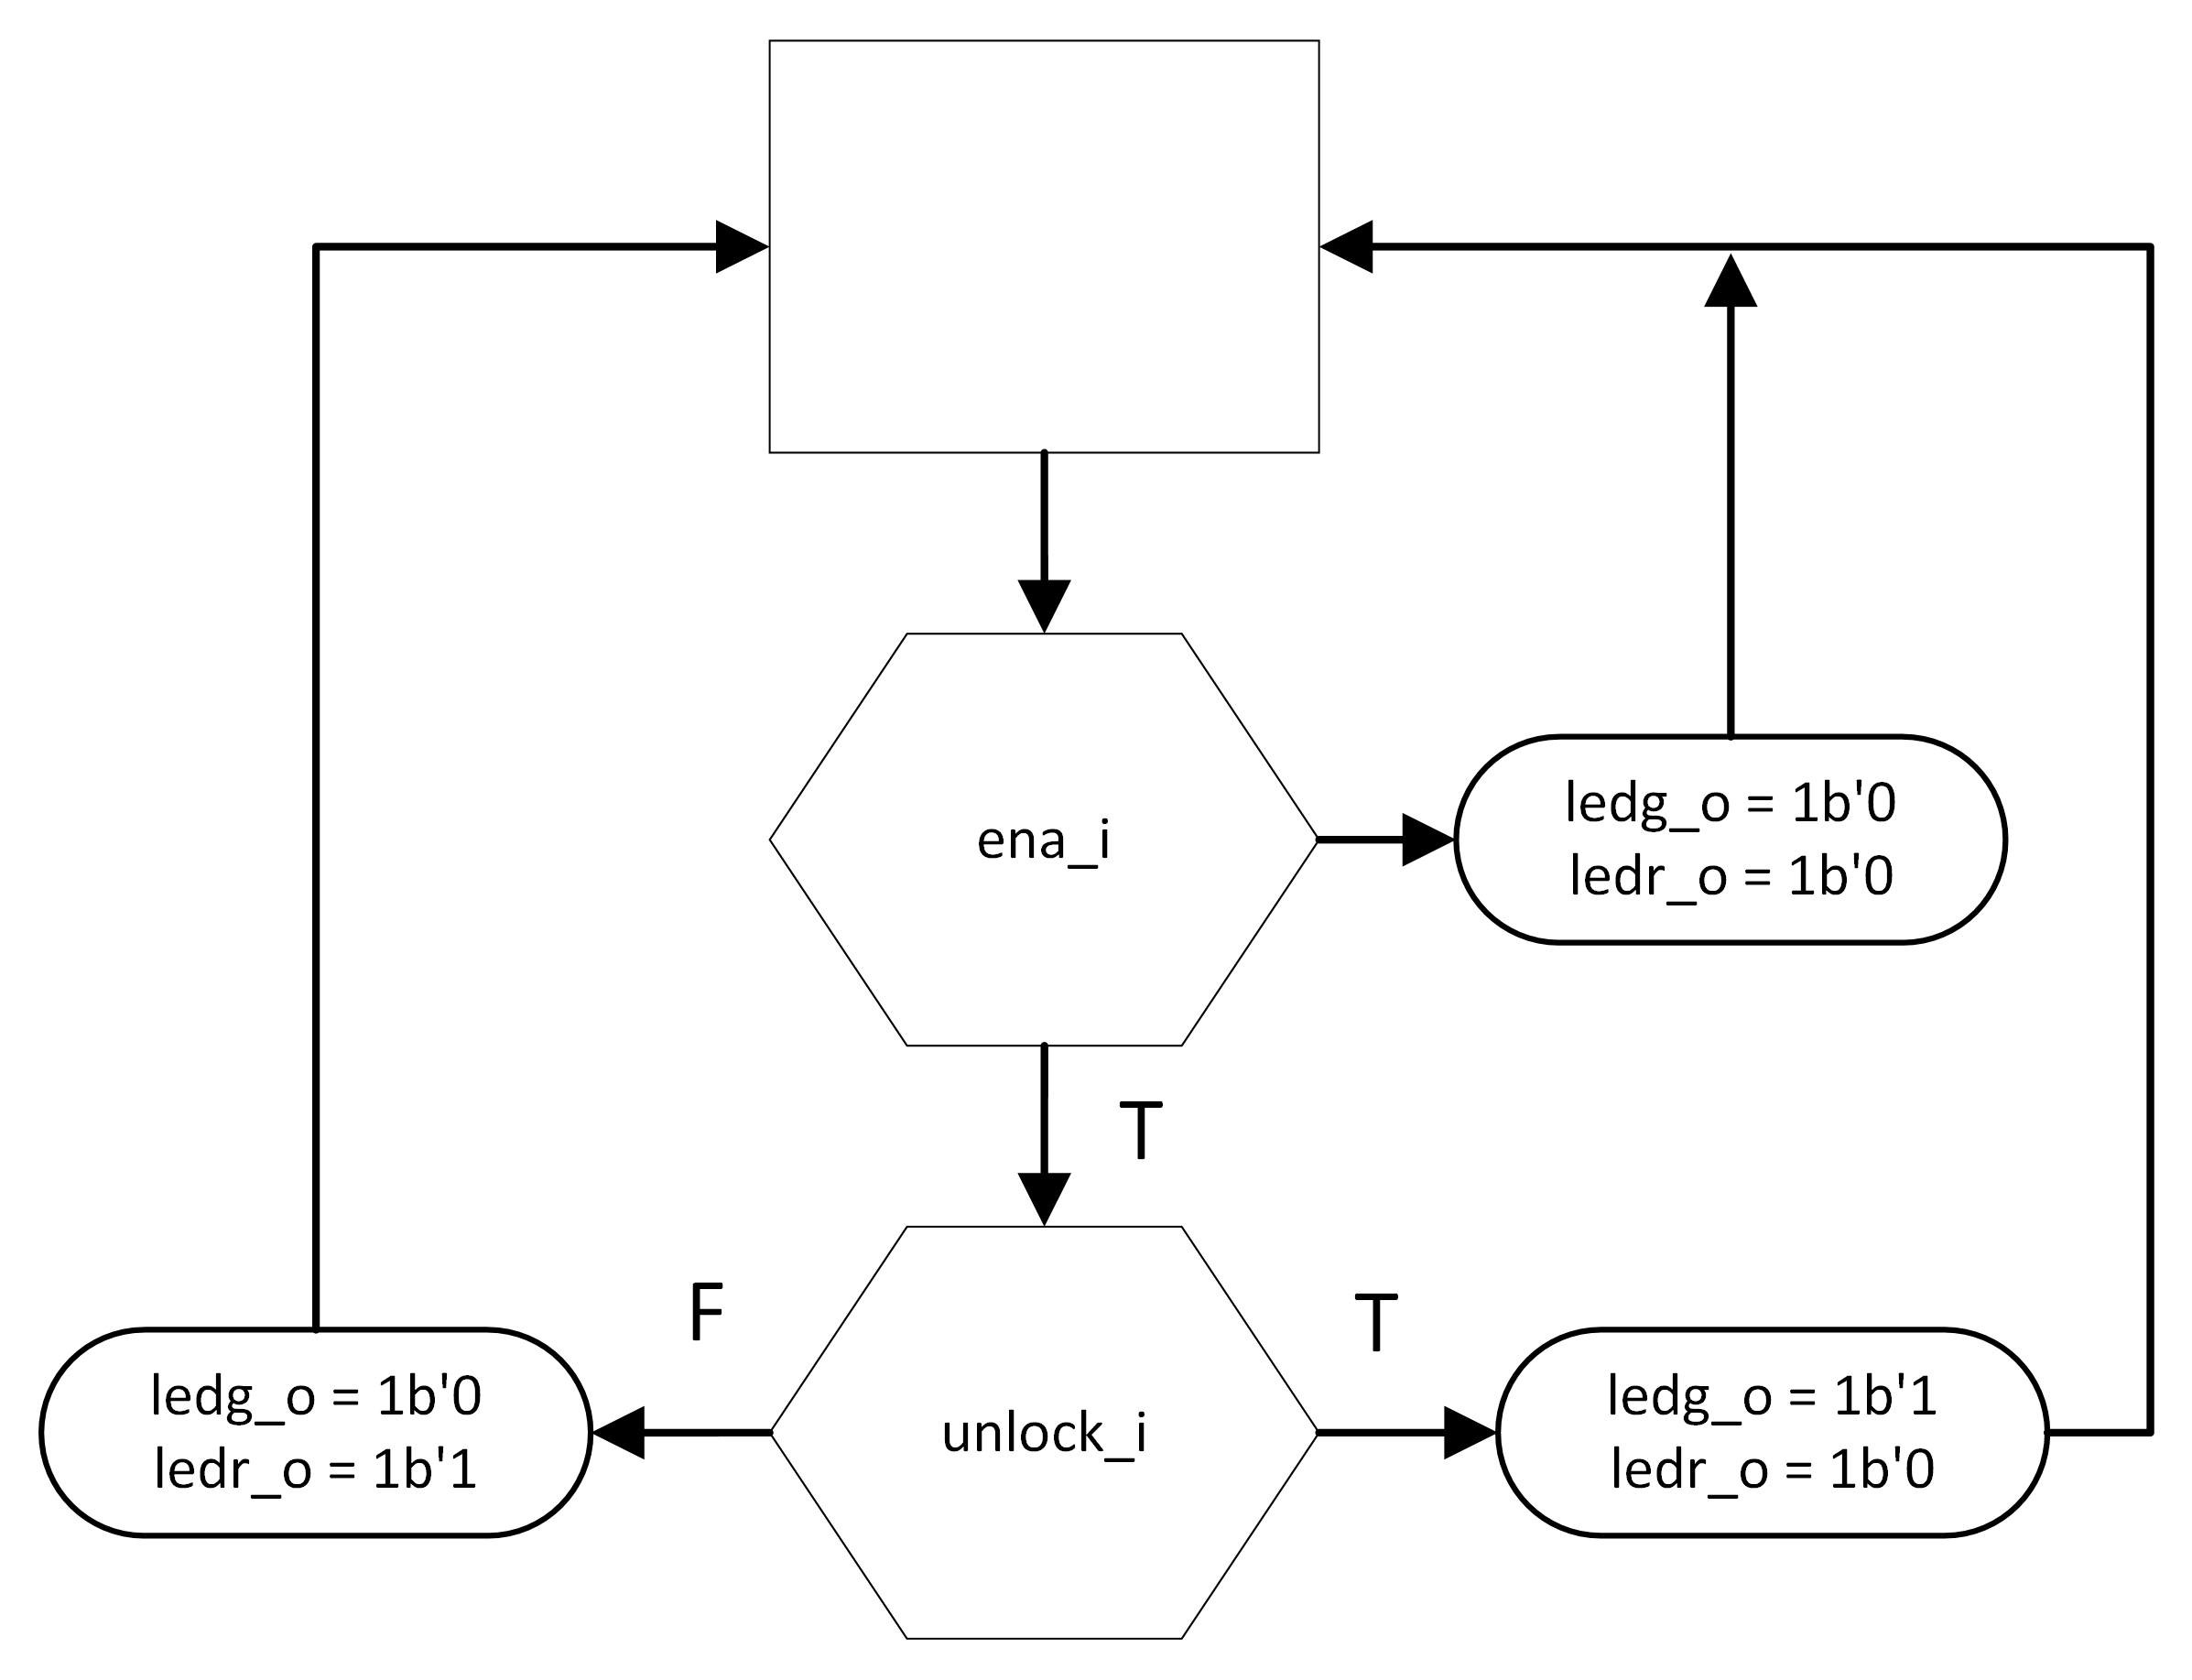
\includegraphics[width=0.85\textwidth]{lock_asm.png}
   \caption{ASM chart of the lock module.}
   \label{fig:lock_asm}
\end{figure}

\begin{minted}[
   fontsize=\footnotesize,
   linenos,
   breaklines,
]{verilog}
module lock (
   input enable_i,
   input unlock_i,
   output reg ledr_o,
   output reg ledg_o
);

always @(unlock_i) begin
   ledr_o = 1'b0;
   ledg_o = 1'b0;
   if (enable_i)
      if (unlock_i)
         ledg_o = 1'b1;
      else
         ledr_o = 1'b1;
end

endmodule
\end{minted}

\begin{minted}[
   fontsize=\footnotesize,
   linenos,
   breaklines,
]{verilog}
module lock_tb;

// Inputs
reg enable_i;
reg unlock_i;

// Outputs
wire ledr_o;
wire ledg_o;

lock DUT (
   .enable_i(enable_i),
   .unlock_i(unlock_i),
   .ledr_o(ledr_o),
   .ledg_o(ledg_o)
);

initial begin
   enable_i = 1'b0;  // disabled
   unlock_i = 1'b0;  // locked
end

initial begin
   #20;

   unlock_i = 1'b1;
   #20;
   unlock_i = 1'b0;
   #20;

   enable_i = 1'b1;  // enabled
   unlock_i = 1'b1;
   #20;
   unlock_i = 1'b0;
   #40;

// Finish the Simulation
   #100;
   $finish;
end

endmodule
\end{minted}

\begin{figure}[htbp]
   \centerline{
   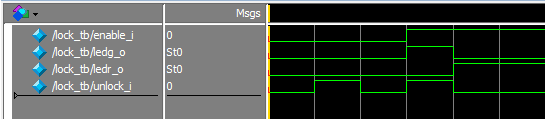
\includegraphics[width=\paperwidth]{lock_sim.png}}
   \caption{Testbench simulation of the lock module.}
   \label{fig:lock_sim}
\end{figure}

Fig.~\ref{fig:lock_sim} is the simulation result of the lock module. The lock turned off both green and red LED when enable signal wa low, turned on the red LED and turned off the green LED when the enable signal is high and unlock signal is low, turned on the green LED and turned off the red LED when the enable signal is high and the unlock signal is high.
